\documentclass[10pt,a4paper]{jarticle}
\usepackage{docmute}
\usepackage{tc2016_utf}
\usepackage[dvipdfmx]{graphicx,color}
\usepackage[fleqn]{amsmath}
\usepackage{algorithm,algorithmic}
\usepackage{amssymb,epsfig}
\usepackage{ascmac}

\usepackage{url}
\usepackage{bm}
\usepackage{ascmac}
\usepackage{pifont}
%\usepackage{multirow}
\usepackage{enumerate}
%\usepackage{cases}
\usepackage{type1cm}
\usepackage{here}
\usepackage{secdot}
\sectiondot{subsection}
\sectiondot{subsubsection}

\DeclareRelationFont{JY1}{mc}{it}{}{OT1}{cmr}{it}{}
\DeclareRelationFont{JT1}{mc}{it}{}{OT1}{cmr}{it}{}
\DeclareFontShape{JY1}{mc}{m}{it}{<5> <6> <7> <8> <9> <10> sgen*min
    <10.95><12><14.4><17.28><20.74><24.88> min10
    <-> min10}{}
\DeclareFontShape{JT1}{mc}{m}{it}{<5> <6> <7> <8> <9> <10> sgen*tmin
    <10.95><12><14.4><17.28><20.74><24.88> tmin10
    <-> tmin10}{}
\DeclareRelationFont{JY1}{mc}{sl}{}{OT1}{cmr}{sl}{}
\DeclareRelationFont{JT1}{mc}{sl}{}{OT1}{cmr}{sl}{}
\DeclareFontShape{JY1}{mc}{m}{sl}{<5> <6> <7> <8> <9> <10> sgen*min
    <10.95><12><14.4><17.28><20.74><24.88> min10
    <-> min10}{}
\DeclareFontShape{JT1}{mc}{m}{sl}{<5> <6> <7> <8> <9> <10> sgen*tmin
    <10.95><12><14.4><17.28><20.74><24.88> tmin10
    <-> tmin10}{}
\DeclareRelationFont{JY1}{mc}{sc}{}{OT1}{cmr}{sc}{}
\DeclareRelationFont{JT1}{mc}{sc}{}{OT1}{cmr}{sc}{}
\DeclareFontShape{JY1}{mc}{m}{sc}{<5> <6> <7> <8> <9> <10> sgen*min
    <10.95><12><14.4><17.28><20.74><24.88> min10
    <-> min10}{}
\DeclareFontShape{JT1}{mc}{m}{sc}{<5> <6> <7> <8> <9> <10> sgen*tmin
    <10.95><12><14.4><17.28><20.74><24.88> tmin10
    <-> tmin10}{}
\DeclareRelationFont{JY1}{gt}{it}{}{OT1}{cmbx}{it}{}
\DeclareRelationFont{JT1}{gt}{it}{}{OT1}{cmbx}{it}{}
\DeclareFontShape{JY1}{mc}{bx}{it}{<5> <6> <7> <8> <9> <10> sgen*goth
    <10.95><12><14.4><17.28><20.74><24.88> goth10
    <-> goth10}{}
\DeclareFontShape{JT1}{mc}{bx}{it}{<5> <6> <7> <8> <9> <10> sgen*tgoth
    <10.95><12><14.4><17.28><20.74><24.88> tgoth10
    <-> tgoth10}{}
\DeclareRelationFont{JY1}{gt}{sl}{}{OT1}{cmbx}{sl}{}
\DeclareRelationFont{JT1}{gt}{sl}{}{OT1}{cmbx}{sl}{}
\DeclareFontShape{JY1}{mc}{bx}{sl}{<5> <6> <7> <8> <9> <10> sgen*goth
    <10.95><12><14.4><17.28><20.74><24.88> goth10
    <-> goth10}{}
\DeclareFontShape{JT1}{mc}{bx}{sl}{<5> <6> <7> <8> <9> <10> sgen*tgoth
    <10.95><12><14.4><17.28><20.74><24.88> tgoth10
    <-> tgoth10}{}
\DeclareRelationFont{JY1}{gt}{sc}{}{OT1}{cmbx}{sc}{}
\DeclareRelationFont{JT1}{gt}{sc}{}{OT1}{cmbx}{sc}{}
\DeclareFontShape{JY1}{mc}{bx}{sc}{<5> <6> <7> <8> <9> <10> sgen*goth
    <10.95><12><14.4><17.28><20.74><24.88> goth10
    <-> goth10}{}
\DeclareFontShape{JT1}{mc}{bx}{sc}{<5> <6> <7> <8> <9> <10> sgen*tgoth
    <10.95><12><14.4><17.28><20.74><24.88> tgoth10
    <-> tgoth10}{}
\DeclareRelationFont{JY1}{gt}{it}{}{OT1}{cmr}{it}{}
\DeclareRelationFont{JT1}{gt}{it}{}{OT1}{cmr}{it}{}
\DeclareFontShape{JY1}{gt}{m}{it}{<5> <6> <7> <8> <9> <10> sgen*goth
    <10.95><12><14.4><17.28><20.74><24.88> goth10
    <-> goth10}{}
\DeclareFontShape{JT1}{gt}{m}{it}{<5> <6> <7> <8> <9> <10> sgen*tgoth
    <10.95><12><14.4><17.28><20.74><24.88> tgoth10
    <-> tgoth10}{}
\endinput
%%%% end of jdummy.def

\def\vec#1{\mbox{\boldmath$#1$}}
\def\vector#1{\mbox{\boldmath $#1$}}

\newcommand{\argmax}{\mathop{\rm arg~max}\limits}
\newcommand{\argmin}{\mathop{\rm arg~min}\limits}
\newcommand{\umax}{\mathop{\rm max}\limits}

\def\R{{\Bbb R}}
\def\Z{{\Bbb Z}}

\renewcommand{\topfraction}{0.8}
\renewcommand{\bottomfraction}{0.8}
\renewcommand{\dbltopfraction}{0.8}
\renewcommand{\textfraction}{0.1}
\renewcommand{\floatpagefraction}{0.8}
\renewcommand{\dblfloatpagefraction}{0.8}
\setcounter{topnumber}{3}
\setcounter{bottomnumber}{3}
\setcounter{totalnumber}{3}
\begin{document}
\section{探索対象の発見課題に対する取り組み}
\label{200657_7Dec16}
課題コース途中で探索エリアにおいて特定人物(探索対象)の発見という課題も設定されている.我々はこの課題を3次元LIDARから得られた3次元点群の処理による実現を試みた.

\subsection{地面点群の除去}
3次元LIDAR(Hokuyo YVT-X002)で得られた3次元点群からまず地面点群の除去を行う.LIDARの取り付け位置は既知であり,つくばチャレンジ2016の課題コースでは探索エリアは平面だったため,地面点群はZ方向の高さによって消去した.
\subsection{クラスタリング}
地面点群が除去された点群をユークリディアンクラスタリングによりクラスタリングを行った.ユークリディアンクラスタリングではある点群からのユークリッド距離がしきい値以下の場合に同一クラスタとする手法である.
\subsection{識別}
クラスタリング後の点群の識別には夏迫ら\cite{chibainst2015}がつくばチャレンジ2015のレポートで提案されていた手法を参考にSVMによる手法を利用した.しかし,特徴量に関しては文献\cite{tokudome2016}の特徴量を用いた.
\subsubsection{点群特徴量}
識別に利用した特徴量$f_{i}$は6次元からなる$f_{i1}$と7次元からなる$f_{i2}$の2つの特徴ベクトルを並べた13次元の特徴量である.
まず,$f_{i1}$は点群の3次元共分散行列の要素であり次式で示される.
\begin{eqnarray}
 \Sigma = \frac{1}{n-1}\sum_{\vec{x_{k}}(i)\in C_{i}}\vec{x}_{k}^{(i)}\vec{x}_{k}^{(i)T}\label{234310_5Dec16}
\end{eqnarray}
ここで,$\vec{x}_{k}^{(i)}\triangleq[x_{k}^{(i)} y_{k}^{(i)} z_{k}^{(i)}]^{T}$はクラスタ内に含まれる点群のクラスタ重心を原点とする座標である.この行列は対称行列であるため,行列要素のうち重複を除いた6要素を特徴量として,$\vec{f}_{i1} = [f_{i11}, \cdots, f_{i16}]^{T}$とする.
式\eqref{234310_5Dec16}に示す3次元共分散行列の固有値を$\lambda_{1}, \lambda_{2}, \lambda_{3}$とする.ただし,$\lambda_{1} < \lambda_{2} < \lambda_{3}$である.この固有値を元にTable.\ref{222525_5Dec16}に示す特徴量を計算しこれを$\vec{f}_{i2}$とした.
\begin{table}
 \centering
 \caption{3D features of points}
 \label{222525_5Dec16}
 \begin{tabular}{|c|c|c|}
  \hline
  $f_{i21}$ & Linearity & $(\lambda_{1}-\lambda_{2})/\lambda_{1}$ \\
  $f_{i22}$ & Planarity & $(\lambda_{2}-\lambda_{3})/\lambda_{1}$ \\
  $f_{i23}$ & Scattering & $\lambda_{3}/\lambda_{1}$ \\
  $f_{i24}$ & Omnivariance & $\sqrt[3]{\lambda_{1}\lambda_{2}\lambda_{3}}$ \\
  $f_{i25}$ & Anisotropy & $(\lambda_{1}-\lambda_{3})/\lambda_{1}$ \\
  $f_{i26}$ & Eigenetropy & $-\sum^{3}_{i=1}\lambda_{i}\ln\lambda_{i}$ \\
  $f_{i27}$ & Change of curvature & $\lambda_{3}/(\lambda_{1}+\lambda_{2}+\lambda_{3})$ \\
  \hline
 \end{tabular}
\end{table}

\subsubsection{SVM}
得られた特徴量をSVM(Support Vector Machine)を用いて識別する.実装にはLIBSVMを利用した.学習はクラスタリングによって得られた点群を287個用意して,それらを探索対象とその他の2値分類問題として行った.学習の結果訓練データで99.3\%,テストデータでも85\%の精度が得られた.

\subsection{探索対象へのアプローチ}
実用上は学習データ数が少なかったこともあり,誤検出が多くなってしまった.そこで,検出位置から1メートル以内で複数回,探索対象と認識した場合にのみアプローチすることにした.
探索対象が見つかった場合には,Fig.\ref{142629_6Dec16}のように探索対象を中心とする円とロボットの自己位置と探索対象を直線結んだ時の交点座標のうち,ロボットに近い方の交点を新たなゴールとして設定する.

\begin{figure}[ht]
 \centering
 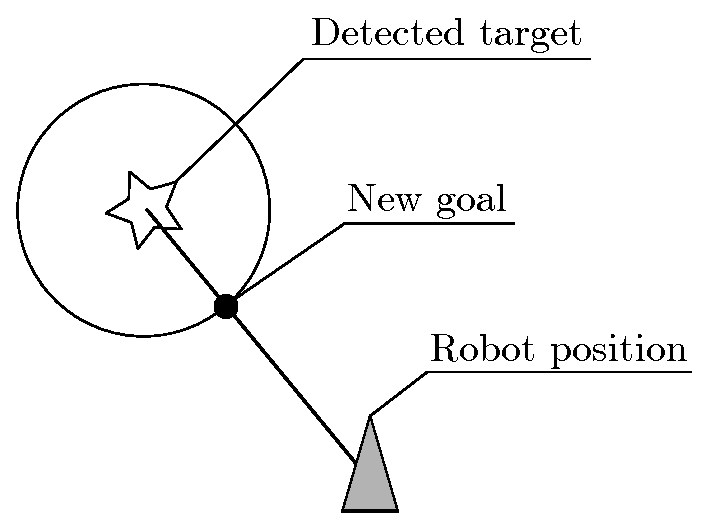
\includegraphics[width=5cm]{./fig/eps/approach_to_target.eps}
 \caption{探索対象へのアプローチ}
 \label{142629_6Dec16}
\end{figure}

以下にこれまでに述べた手法をまとめる.
\begin{enumerate}
 \item 3DLIDARによって得られた点群から地面点群を除去する
 \item 地面点群が除去された点群をクラスタリングする
 \item クラスタリング結果をSVMによって識別し,探索対象ならアプローチ候補とする
 \item アプローチ候補のうち,1m以内で複数回アプローチ候補が検出された場合にアプローチ対象とする
\end{enumerate}

\subsubsection{人物探索のつくばチャレンジにおける実験結果}
これまでに説明した手法は九州工業大学戸畑キャンパス内に設定したコース内では上手く機能していた.しかし,試験走行日にこれらを実際に試してみたところ,学内で実験した場合よりも多く誤認識してしまい,それら全てにアプローチを試みるという結果になってしまった.そのため,制限時間内で課題コースを完走することが難しいと判断し,本走行では人物探索機能を起動させなかった.
課題コースでは建物の角などを探索対象として多く誤認識してしまっていた.学内で得られたサンプルには建物の角など人工物があまり含まれておらず,結果としてそれらを上手く識別できていなかったと考えられる.すなわち,学習に用いたデータが少なすぎたことが問題だと考えられる.

\end{document}

% Local Variables:
% mode: yatex
% TeX-master: "tc2016_third.tex"
% End:
